\documentclass[a4paper]{article}
\usepackage[utf8]{inputenc}
\usepackage{booktabs}
\usepackage{rotating}
\usepackage{hyperref}
\usepackage{color, colortbl}
\usepackage{pdfpages}
\usepackage[left=2cm,right=2cm,top=1.5cm]{geometry}

\definecolor{Gray}{gray}{0.9}



\begin{document}
\thispagestyle{empty}

\begin{center}
	\Large
	Technische Universität Dortmund\\
	Fakultät Statistik\\
	Wintersemester 2023/24\\
	
	\vspace{6em}
	
	Erhebungstechniken: Bericht über Fragebogenstudie
	
	\Huge
	\textbf{Lernortsituation an der TU Dortmund}
	
	\Large
	\vspace{4em}
	DozentInnen:	\\Prof. Dr. Philipp Doebler \\Loreen Sabel, M.Sc.\\Hannah Bartmann, B.Sc.


	\vspace{6em}
	Verfasser: \\
	Yannick Miguel \\Jacqueline Link
	
	\vspace{6em}
	Gruppenmitglieder:\\
	Johanna Hohmann\\
	Lisa Larrass
	
    \vspace{6em}
    
	31.01.2024
\end{center}

\newpage \null\thispagestyle{empty}\newpage
\tableofcontents
\newpage\null\thispagestyle{empty}\newpage
Zusammenfassung (bis zu 250 Wörter)
\newpage\null\thispagestyle{empty}\newpage
7-9 Seiten Bericht
\newpage Literaturverzeichnis
\newpage 
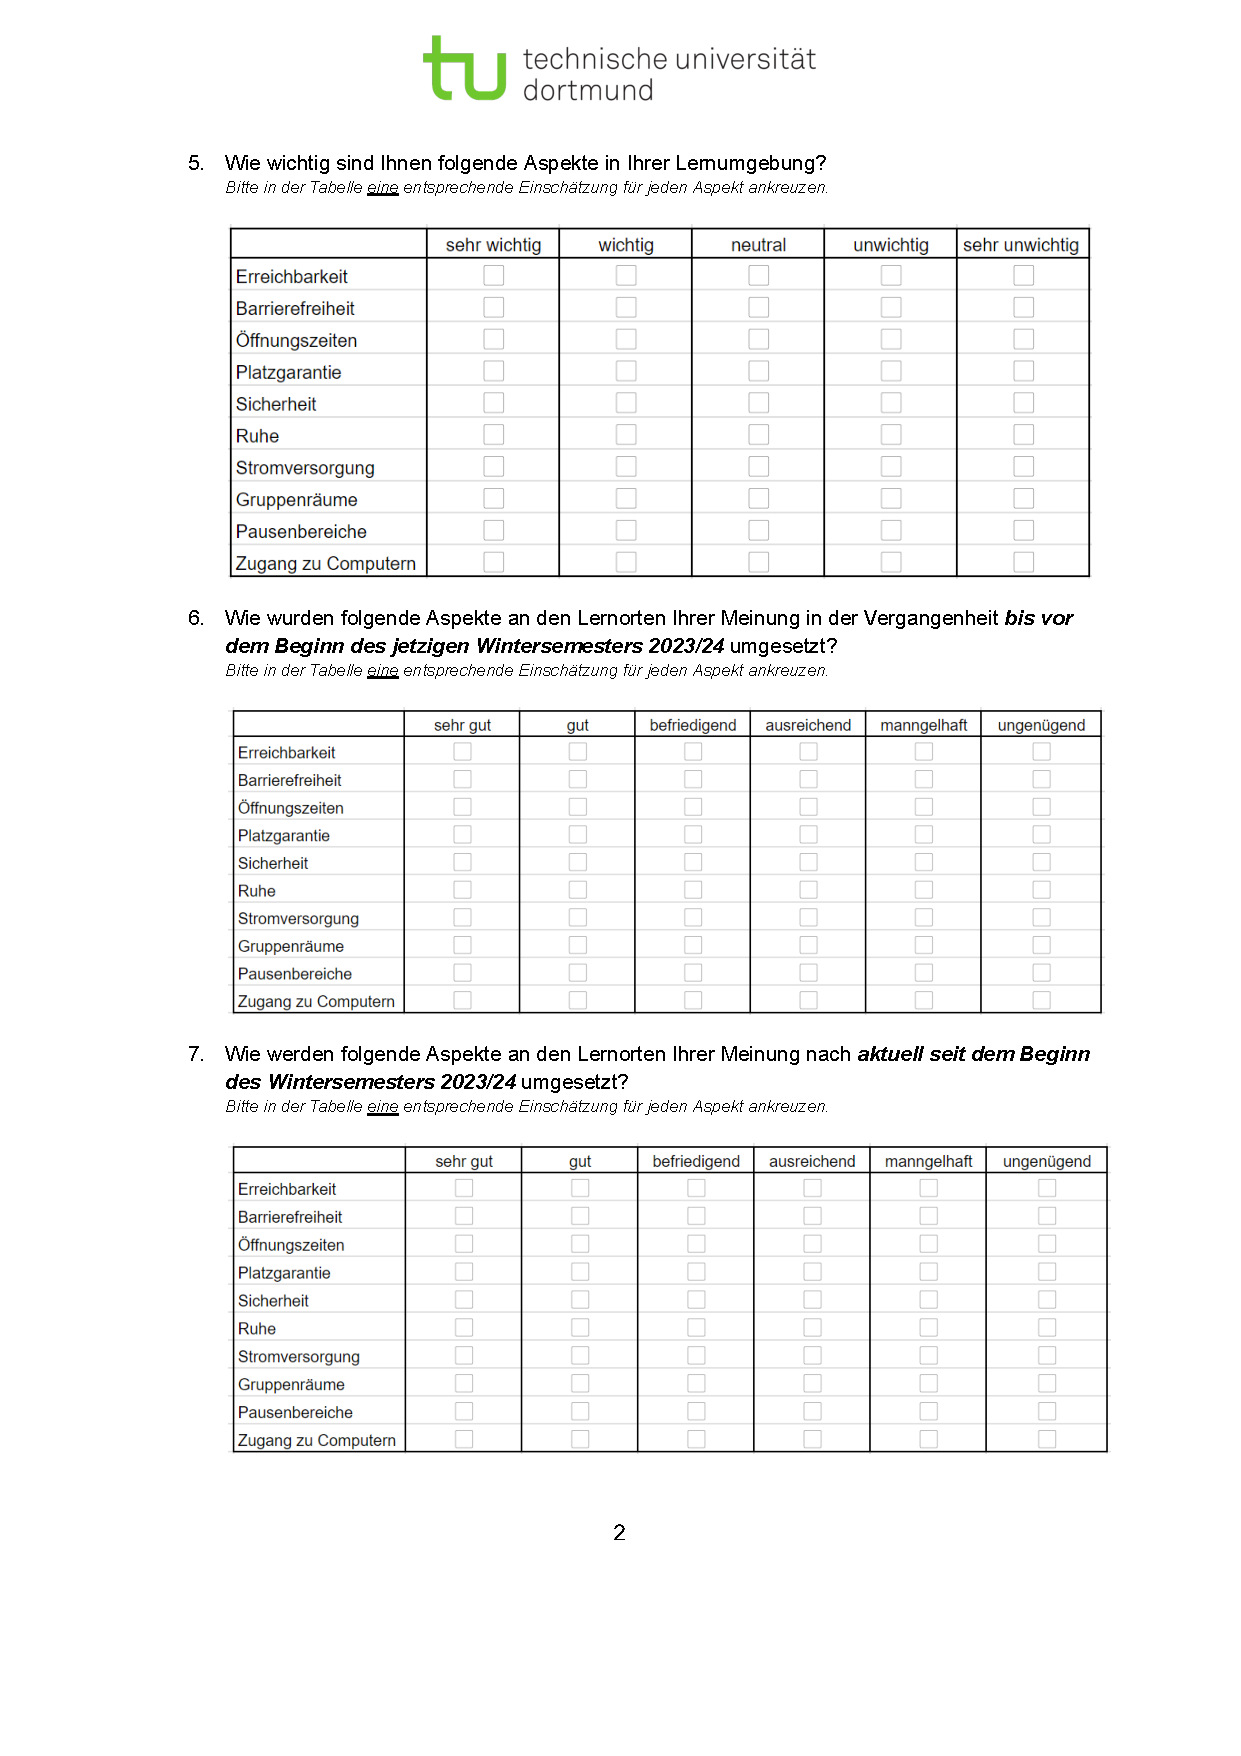
\includepdf[pages=1-4] {C:/Users/yanni/Desktop/Studium/3. Semester/Erhebungstechniken/Fragebogen Projekt/Final.pdf}
\newpage Appendix: Erklärung zu Anteilen an der Textproduktion

\end{document}



